\problemname{Claw Machine}
Olivia and Anton are at Liseberg, 
where they've found a claw machine with $N$ stuffed animals, 
numbered from $1$ to $N$. 
Olivia is highly skilled and wants to show off her abilities to Anton. 

The two-dimensional claw machine can be modeled as a grid of size $R \times C$, 
with $R$ rows and $C$ columns. 
The stuffed animals are packed tightly, 
with each cell of the grid belonging to one stuffed animal. 
There are no empty cells in the grid.
A stuffed animal may consist of several connected cells in the grid, 
forming a contiguous shape. 
In other words, you can draw each stuffed animal with a thick pen without lifting it from the paper.

In a single move, 
Olivia can choose a stuffed animal that does not have any other stuffed animal directly above it and lift it out of the claw machine. 
Since Olivia hasn't asked Anton about his favorite animal yet, 
she wants to know, for each stuffed animal, 
how many moves she will need to make in total before she can lift it.

\section*{Input}
The first line contains the integers $N$, $R$, and $C$ ($1 \leq N \leq R \times C \leq 4 \times 10^5$).  
The next $R$ lines describe the grid. 
The first line corresponds to the top of the claw machine, 
and the last line corresponds to the bottom.  
The $i$-th rows contains $C$ integers $a_{i,1}, a_{i,2}, ..., a_{i,C}$ ($1 \leq a_{i,j} \leq N$).  
Stuffed animal number $x$ consists of all cells $(i, j)$ such that $a_{i,j} = x$.  
It is guaranteed that each stuffed animal consists of at least one cell and forms a contiguous region.

\section*{Output}
For each stuffed animal $1, 2, ..., N$, 
print the number of moves Olivia needs to make before she can lift that animal. 
If it is not possible, print $-1$.

\section*{Scoring}
Your solution will be tested on a set of test groups, each worth a number of points. Each test group contains
a set of test cases. To get the points for a test group you need to solve all test cases in the test group.

\noindent
\begin{tabular}{| l | l | p{12cm} |}
  \hline
  \textbf{Group} & \textbf{Points} & \textbf{Constraints} \\ \hline
  $1$    & $10$       & $1 \leq N \leq R \times C \leq 20$ \\ \hline
  $2$    & $5$        & $C = 1$ \\ \hline
  $3$    & $10$       & $C \leq 2$ \\ \hline
  $4$    & $15$       & Each stuffed animal has a rectangular shape. \\ \hline
  $5$    & $15$       & $N \leq 2000$ \\ \hline
  $6$    & $7$        & $N \leq 50000$ \\ \hline
  $7$    & $38$       & No additional constraints. \\ \hline
\end{tabular}

\section*{Explanation of Sample 1}
In sample 1, the claw machine looks like this:

\begin{figure}[h!]
  \centering
  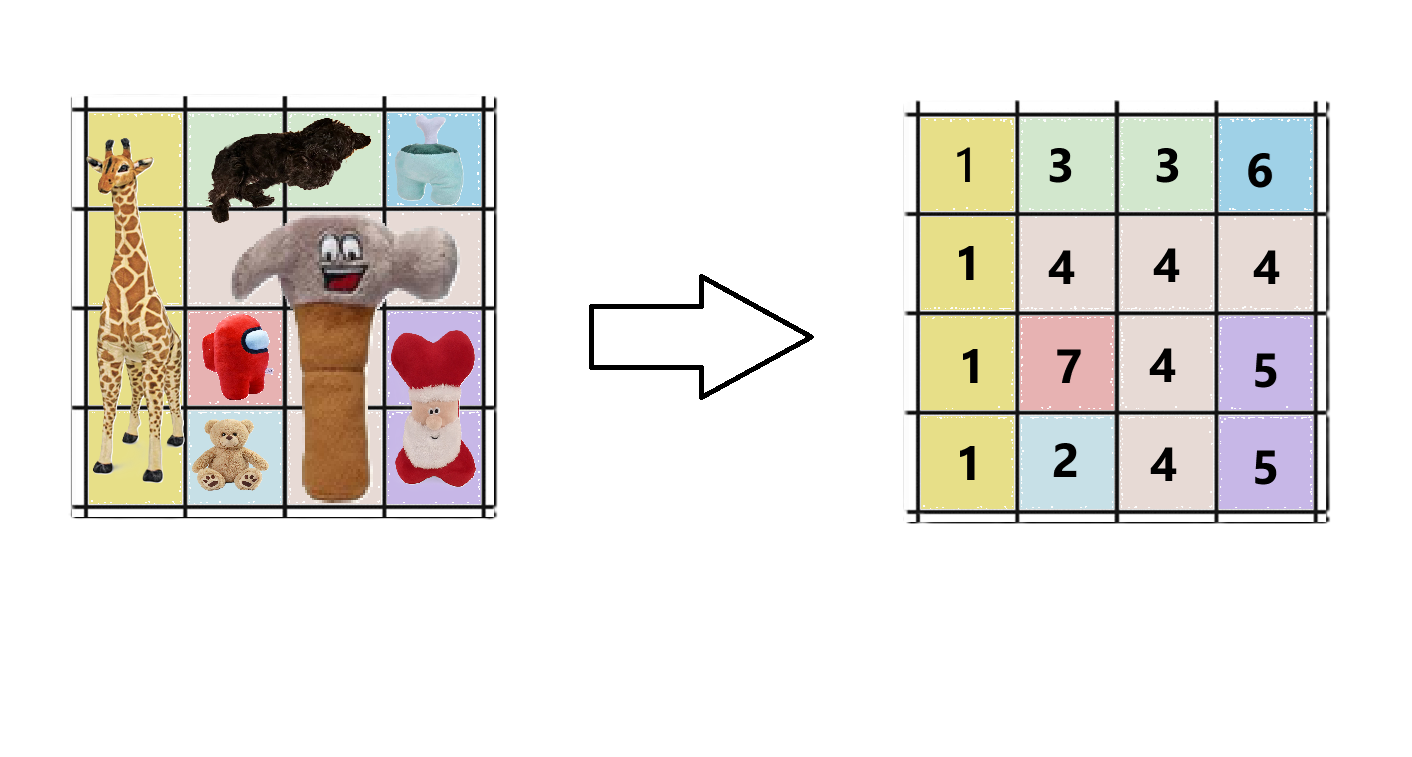
\includegraphics[width=0.5\textwidth]{example.png}
\end{figure}

To lift stuffed animal $1$, no other animal needs to be lifted first, so the answer is $0$.  
To lift stuffed animal $2$, Olivia first needs to lift $3$, $4$, $6$, and $7$, so the answer is $4$.  
To lift stuffed animal $3$, no other animal needs to be lifted first.  
To lift stuffed animal $4$, Olivia needs to lift $3$ and $6$ first, so the answer is $2$.  
The answers for stuffed animals $5$, $6$, and $7$ are $3$, $0$, and $3$, respectively.

Here is how it looks after lifting stuffed animal $3$:

\begin{figure}[h!]
  \centering
  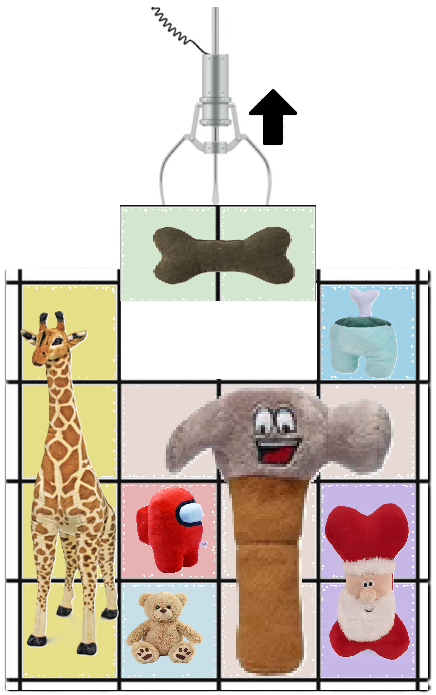
\includegraphics[width=0.35\textwidth]{example2.png}
\end{figure}

\section*{Explanation of Sample 4}
Neither stuffed animal $1$ nor $2$ has anything above them, so the answers for both are $0$.  
To lift stuffed animal $3$, Olivia first needs to lift $4$, but to lift $4$, she needs to lift $3$, creating a loop.  
Thus, the answer for both $3$ and $4$ is $-1$, as it is impossible to lift them.
